\subsection{仿射韦伊群与完备 Dynkin 图}

设 R 是不可约约化根系，\((\mathbf{X}, f)\) 是其 Dynkin 图。我们将定义另一个赋范图 \((\tilde{\mathbf{X}}, \tilde{f})\)，称为 R 的完备 Dynkin 图。\(\tilde{I}\) 是 \(\tilde{X}\) 的顶点集，由 X 的顶点集 I 和一个记为 0 且不属于 I 的顶点组成。为定义 \(\tilde{f}\)，选取 R 的一组基 \(B = (\alpha_{i})_{i \in I}\) 以及在 W(R) 下不变的标量积 \((x|y)\)。令 \(\alpha_{0}\) 为相对于 B 所定义的序的最高根的负根。两个不同顶点 \(i, j \in \tilde{I}\) 相连，当且仅当 \((\alpha_{i}|\alpha_{j}) \neq 0\)，并置

\[
\tilde {f} (i, j) = \frac {\left(\alpha_ {i} \mid \alpha_ {i}\right)}{\left(\alpha_ {j} \mid \alpha_ {j}\right)}.
\]

立即可见，这样定义的图 \(\tilde{X}\) 和映射 \(\tilde{f}\) 不依赖于 B 或标量积的选择。

若秩 \(l\) 的 \(R\) 等于 1，则 \(I = \{i\}\) 且 \(\alpha_0 = -\alpha_1\)；故 \(\tilde{f}(0, i) = 1\)。若 \(l \geqslant 2\)，\(\alpha_0\) 不与任何 \(\alpha_i\) 成比例，且 \((\alpha_0|\alpha_i)\) \(\leqslant 0\)（第 1 节，第 8 号，命题 25）。对于任意一对不同元素 \((i,j)\)（属于 \(\tilde{I}\)），唯一可能性就是前一号中标为 1）、2）、3）、4）的那些可能性（例如置 \(n_{0i} = n(\alpha_0, \alpha_i)\)，\(m_{0i} = \text{阶 } s_{\alpha_0}s_{\alpha_i}\)，其中 \(i \in I\)）。

在 \(l \geqslant 2\) 的情形，完备 Dynkin 图用与前一号相同约定的图表示，有时用虚线表示连接顶点 0 与其他顶点的边。注意，若这种边上存在不等号 \textgreater{}，它总是指向异于 0 的顶点，因为 \(\alpha_{0}\) 是最长根（\(\S\) 1，第 8 号，命题 25）。图 \((\mathbf{X}, f)\) 是从 \((\tilde{\mathbf{X}}, f)\) 删除顶点 0 后得到的子图。

A(R) 在 (X. f) 上的作用延拓为 \((\tilde{\mathbf{X}}.\tilde{f})\) 上的作用，并固定 0；而 W(R) 在 \((\tilde{\mathbf{X}}.\tilde{f})\) 上平凡作用。

我们沿用第 2 节的记号。第 2 节第 2 号的命题 5，连同第五章第 3 节第 2 号的定理 1，表明，仿射韦伊群的 Coxeter 图 \(\Sigma\) 与 \(W_{a}(R)\) 相关；它可以从 \((\tilde{X},\tilde{f})\) 按照由 \(W(R)\) 从 \((X,f)\) 得到其 Coxeter 图的相同规则得到。另一方面，令 G 为 \(W_{a}(R)\) 的正规化子（第 2 节，第 3 号）。对每个 \(g\in G\)，都有一个自同构 \(\varphi(g)\) 作用于 \(\Sigma\)，且 \(\varphi(g)=\mathrm{Id}\)（若 \(g\in W_{a}(R)\)）。反过来，给定 \(\lambda\)，它是 \(\Sigma\) 的一个自同构；根据第五章第 4 节第 9 号的命题 11，存在唯一元素 \(g=\psi(\lambda)\)，保持给定小室 C，并满足 \(\varphi(g)=\lambda\)。由于 G 是保持 C 的元素所成的子群 \(G_{C}\) 与 \(W_{a}(R)\) 的半直积（第 2 节，第 3 号），故 \(\varphi\) 通过取商定义了从 \(G/W_{a}\)（或从 \(G_{C}\)）到 \(\operatorname{Aut}(\Sigma)\) 的同构。立即可见，这个同构与从 A(R)/W(R) 到 G/ \(W_{a}\) 的典范映射的复合，恰好是从 A(R)/W(R) 到 \(\operatorname{Aut}(\Sigma)\) 的同态；这个同态由上面定义的从 A(R)/W(R) 到 \(\operatorname{Aut}(\tilde{X},\tilde{f})\) 的同态所诱导。根据第 2 节第 3 号，群 \(\operatorname{Aut}(\Sigma)\) 同构于

\(A(R)/W(R)\) 与 \(P(R')/Q(R')\) 的半直积，而 \(P(R')/Q(R')\) 同构于群 \(I_{C'} = G_{C'} \cap W_{a}'\)（记号同第 2 节第 3 号）：\(\text{Aut}(\Sigma)\) 中与 \(\gamma_{i}\)（\(I_{C}\) 中的元素）相对应的元素，将顶点 0 变为 \(\Sigma\) 的顶点 i。

备注。可以证明，典范映射

\[
\operatorname{Aut} (\tilde {X}, \tilde {f}) \rightarrow \operatorname{Aut} (\Sigma)
\]

是一个同构。

定理 4. 设 (W.S) 是 S 有限的不可约 Coxeter 系统。关联的二次型（第五章第 4 节第 1 号）正且退化，当且仅当 (W.S) 的 Coxeter 图同构于下列图之一：

\pandocbounded{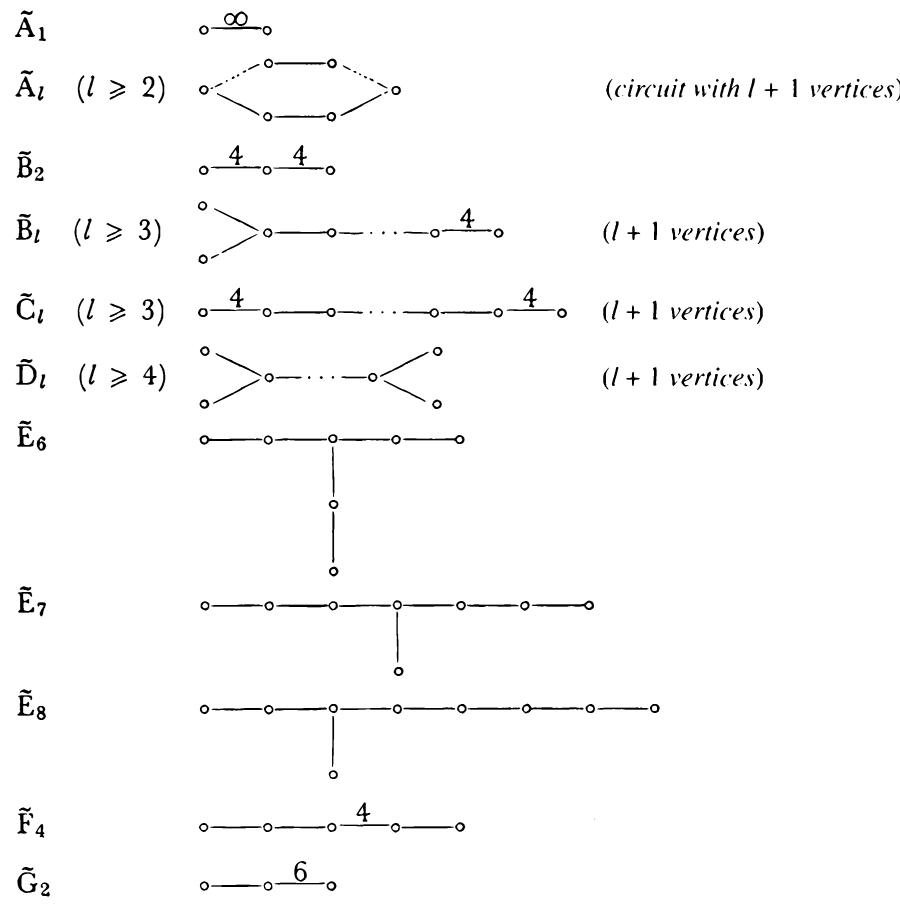
\includegraphics[keepaspectratio]{images/part002_b5f8d83f.jpg}}

这些 Coxeter 图中任意两个都不同构。

根据第五章第 4 节第 9 号以及第 2 节第 5 号的命题 8，二次型正且退化的 Coxeter 系统正是对应于不可约约化根系的仿射韦伊群的那些系统。因此，定理由下面第 5 至 13 号中对完备 Dynkin 图的确定得出。

